\documentclass[10pt,a4paper]{report}
\title{Cryptography Report}
\author{Michele Orr\`u}

\usepackage[
  a4paper,
  inner=1.5cm, outer=1.5cm,
  top=3cm, bottom=3cm,
  bindingoffset=1cm]{geometry}
\usepackage[
  font=small,
  format=plain,
  labelfont=bf,up,
  textfont=normal,up,
  justification=justified,
  singlelinecheck=false]{caption}

\usepackage{amsmath}
\usepackage{amsthm}
\usepackage{float}
\usepackage{minted}
\usepackage{graphicx}
\usepackage{wrapfig}

\newcommand{\code}[1]{\texttt{#1}}
%% REPORT INSTRUCTIONS:
%% --------------------
%%
%% Write a REPORT about the lab project
%% covering the following points:
%%
%% - Describe your integer pseudorandom generator.
%% - Describe your prime pseudorandom generator.
%% - Describe how you generated the RSA keys, specifying:
%%   - which controls you made on the primes;
%%   - an estimate of the time and of how many integers
%%     you have to check to generate 512 bit primes
%%     with your own prime pseudorandom generator.
%% - Describe how you generated the symmetric keys.
%% - In the protocol proposed in the course there may be dome flawes:
%%   please elaborate.
%%
%% Report length must be:
%% at most 2 pages (+2 of cited code/pseudocode/pictures if needed)
%% Clarity in the exposition will also be evaluated.
%%


\begin{document}
\maketitle

\section{Pseudorandom integers generation}
A pseudorandom number generator (from now on simply called PRNG), consists in an
algorithm generating a sequence of numbers that approximate the properties of a
random number. Reacalling \cite{stallings}, these properties are:
\begin{itemize}
  \setlength{\itemsep}{1pt}
  \setlength{\parskip}{0pt}
  \setlength{\parsep}{0pt}

\item uniformity: at any point of the sequence, the number of zeroes and ones is
  equally likely;
\item scalability: any test applicable to a sequence can be applied to random
  subsequences;
\item consistency: the behaviour of the generator must be consistent across
  starting values.
\end{itemize}

\noindent
Moreover, the algorithm must be checked against a potentially infinite number of
statistical tests, before asserting that also the implementation is correct. In
our case, we restricted among some of the most common and
widespread ones\cite{beautifultesting}: $\mu$-test, $\sigma^2$-test, bucket-test, and
KS-test.


\subsection{Fast Random Number Generation}

First of all we recall the definition of a fast PRNG:

\newtheorem*{FPRNG}{Definition}
\begin{FPRNG}
  A Fast PRNG is an algorithm generating a random sequence of integers with good
  statistical properties.
\end{FPRNG}

On the basis of the previous lessons, it would be straightforward to use any
stream cipher, which by construction have all really good statistical
properties, and prove that the period of such a random number generator is
bigger than the maximum value of a \code{size\_t} type.
Though, for performance reasons, we used instead a trivial implentation of a Mersenne
Twister.

\subsection{Safe Random Number Generation}

Again, we start by recalling the prequisites for a secure PRNG:

\newtheorem*{SPRNG}{Definition}
\begin{SPRNG}
  A safe PRNG satisfies ``good'' statistical properties and the security
  constraint that from the output bits the initial state cannot be recovered.
\end{SPRNG}

Here, assuming that the word ``good'' means ``approximating a uniform
distribution'', and considering that BUNNY24 is the ideal cipher, then any
message encrypted with BUNNY24 is perfectly random.

\begin{proof}

Let $c$ be the random stream generated by our Secure PRNG $g$.\\
Let $k \in K$ be the seed. \\
Let $m$ be a constant stream of bytes. \\
We want to show that if $g$ is based on a perfect cipher $\varphi$, then
(1) all seeds are equally likely,
(2) different seeds will give different output streams.

If we construct $g_k$ so that $c = g_k = \varphi_k(m)$, we are done. By
hypothesis, $\varphi_k$ is the perfect cipher. This implies, under Shannon's
Theorem,
\begin{align}
P(k_1) = P(k_2) \ \ \forall k_1, k_2 \in K   \\
\exists!k\ .\ \varphi_k(m) = c
\end{align}



\end{proof}

Specifically, we configured the PRNG so that the message is a stream of
\code{NUL} bytes, the key corresponds to the first three bytes of the seed, and
the IV is the last byte of the seed padded with \code{NUL} bytes.

\subsection{Prime Random Number Generation}

The prime number generation consists into a simple wrapper around the Secure
PRNG. It continuosly generates odd random \code{BIGNUM}s (i.e. interpreting the
random bytestream as a \code{BIGNUM} structure), until the one that passes $10$ tests
for primality is found.
\footnote{Note that, as 1 is not considered prime, this
  excludes all possible corner-cases of returning values like $0$, $1$, $2$.}
The function has been implemented as follows:
\begin{minted}{c}
/**
 * \brief A "safe" prime random number generator.
 *
 */
BIGNUM* prng(BIGNUM** p, int bits)
{
  do {
    bn_rng(p, bits);
    if (!BN_is_odd(*p)) BN_add(*p, *p, BN_value_one());
  } while (!BN_is_prime(*p, 10, NULL, NULL, NULL));

  return *p;
}

\end{minted}
In the following section, there will be a discussion on how the \emph{seed} has
been fetched, and used.

\section{Keys Generation}

Generating keys for any cipher (symmetric or asymmetric) requires a good entropy
source. This is impossible to achieve, neither relying on the primitives
developed during the course lectures, nor relying on the user himself - humans
are not good entropy sources. Hence, we decided to take advantage of some
kernel’s features, i.e. the two special files \code{/dev/random} and
\code{/dev/urandom}.
They both gather randomness from device drivers into an entropy pool, from which
random numbers are created.
Though, the first mentioned returns only random bytes within the estimated
number of noise bits in the entropy pool, while the second one will not stop waiting
for more entropy.

Both sources were used just as seeds for generating a longer bytestream using
the Secure PRNG, but \code{/dev/random}, being a slow blocking device has been
opened only for long-lived random RSA keys.

\subsection{RSA Keys Generation}

RSA keys generation consists in finding (i) two primes $p, q$ and (ii)
two integers $e, d$ such that \linebreak $ed \equiv 1 \pmod{\varphi(pq)}$.

\begin{figure}[h!bt]
  \centering
  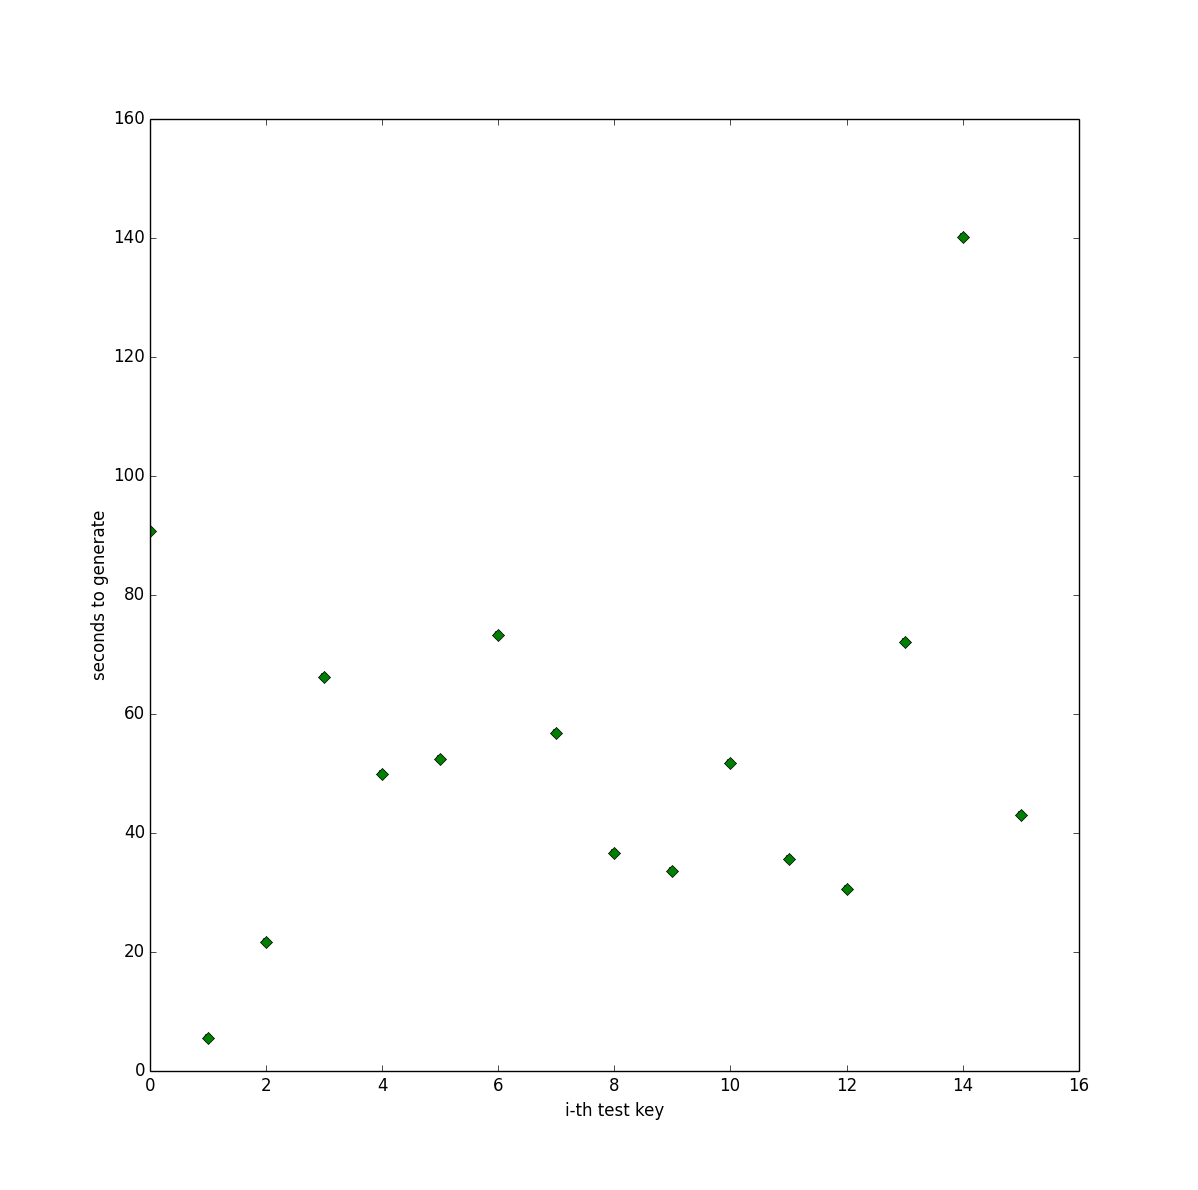
\includegraphics[scale=.27]{dataset512.png}
  \caption{RSA-512 benchmarking. \label{fig:rsa512}}
\end{figure}


Following the security threats emerged in Lecture 3, the two primes where
generated asserting that \linebreak $\log p \approx \log q$.  Also, in order to
avoid attacks such as \emph{Pollard's $p-1$ Attack}, the primes $p$ and $q$ were
actually chosen among safe primes.
\footnote{A prime p is said to be a safe prime ifff $\frac{p-1}{2}$ is prime}
After a few test samples, it emerged that on average there is only one safe
prime number every 272 primes.
Lastly, in order to avoid low-public exponent attacks, the public key was
selected to be of $keysize - 1$ bits.
\footnote{
  At the current revision, there isn't any check on the private
  exponent. This could lead to attacks such as Wiener's, if
  $ d < \frac{1}{3}N^\frac{1}{4} $}

Our implementation takes about $53.74$ seconds on average to generate a
valid RSA512 key.\footnote{Tests were performed on a \code{x86-64 Intel i7 @ 2000 GHz}}

\subsection{Symmetric Keys Generation}

According to the protocol specifications, symmetric keys exchange must be
performed using RSA encryption with a cryptographically secure random token.
This imposes a few constraints: it must be generated using the secure PRNG and
it must be of length greater or equal than three bytes.
Note that tokens of a bigger size will not provide stronger security.

In our case, we are transmitting a random \code{BIGNUM} of 16-bits of size.


\section{Protocol Flaws}

Excluding feasible \emph{bruteforce attacks} on the symmetric cipher, our current
use of RSA could be vulnerable to \emph{timing attacks}.
It is indeed possible, assuming Eve can listen to both \code{client} and
\code{server}, to retrieve information about the length of the messages
sent/received, since our encryption function is not time-constant but its
computation strongly depends on the given input.

Looking at the protocol from a communicative perspective, we notice that using
FIFOs as a transport layer is a really bad choice.
FIFOs are not meant to be used in a scenario like the server/client one: the
existence of better data structures, like Unix Sockets, provides a more
efficient, secure, full-duplex communication.
Using an external FIFO file as transport layer delegates all the security to its
permissions as a file, which are not being checked at startup.  This potentially
exposes the application to \emph{eavesdropping} - if the file is readable,
\emph{dossing} and \emph{plaintext attack} - if the file is writable.



\begin{thebibliography}{9}
  \bibitem{stallings}
    Stallings,
    \emph{Cryptography and Network Security}

  \bibitem{nist-rng}
    NIST,
    \emph{SP800-22},
    2001
  \bibitem{beautifultesting}
    O'Reilly,
    Tim Riley \and Adam Goucher,
    \emph{Beautiful Testing: \
      Leading Professional Reveal How They Improve Software},
    2010
\end{thebibliography}

\end{document}
